\documentclass[10pt,twocolumn, a4paper]{article} 
\title{Combination of SVM and FERN for GPU-assisted texture recognition on mobile devices}
\usepackage[cm]{fullpage}

\usepackage{float} 
\usepackage{algpseudocode}
\usepackage{graphicx}
\usepackage{mathrsfs}
\usepackage{bbm}
\usepackage{mdwlist}
\usepackage[lofdepth,lotdepth]{subfig}
\usepackage{amsmath}
\usepackage{multirow}

\DeclareMathOperator*{\argmin}{arg\,min} 
\DeclareMathOperator*{\argmax}{arg\,max} 
\author{Vsevolod Yugov\thanks{Tokyo Institute Of Technology, Dept. of Information Processing}, Itsuo Kumazawa\thanks{Dr. of Engineering,
Imaging Science and Engineering Laboratory 
Tokyo Institute of Technology 
}}

\begin{document}
\maketitle

\begin{abstract}
Feature point matching and texture recognition are two of the most important problems in the image processing. Recently, several new approaches to these problems using simple local features and semi-naive Bayesian classification scheme have been developed. In our paper, we show how to enhance these techniques further by combining them with Support Vector Machines using online learning techniques. The resulting algorithm is simple, robust and can be adapted to various tasks in image processing. Furthermore, we demonstrate the advantages of our method by using it to achieve real-time texture recognition on a mobile device by utilizing parallel processing capabilities afforded by the device GPU.
\end{abstract}

\section{Introduction}
\label{Intro}
Image processing and computer vision on the mobile devices are rapidly developing topics due to the increased processing power available. In particular, many modern devices are equipped with programmable GPU, allowing for parallel computation over the whole image. The drawback of using GPU lies in the fact that many state-of-the art image-processing algorithms are employing sophisticated features that are too complex to be processed with the limited resources available for a single thread during parallel execution. Due to this limitation, algorithms using extremely simple features, like Ferns (\cite{Ferns1}, \cite{Ferns2}) or Local Binary Patterns (\cite{LBP}) are preferable. Such algorithms have been successfully adapted to mobile tracking problem in \cite{Mobi}, however, it has been noted that the accuracy is degrading rapidly as the number of features is decreased.
In our work, we concentrate on improving the accuracy of the method named Ferns, presented in \cite{Ferns1} and \cite{Ferns2}, which uses non-hierarchical structures consisting of a small number of random binary tests to estimate probability of an image patch belonging in a certain class. Several of such structures are later combined in a Naive Bayesian way. 
We first consider a simple case of binary classification problem, which allows using Ferns algorithm for object and texture detection, similar to \cite{LBP}, which is our focus in this paper.  Later we show how our algorithm can be expanded for multiple classes, allowing its usage in keypoint classification.
We first replace the Naive Bayesian combination by a weighted Bayesian approach. In order to calculate weights we use online training algorithm for Support Vector Machines described in \cite{Norma}, for the merits of its simplicity and low computational cost.
We also evaluate and compare efficiency and resulting accuracy of using probabilities, logarithmic likelihoods or binary thresholding for likelihood calculation. Our results indicate, that application of this method can achieve significant increase in accuracy compared to original Ferns, and that using binary thresholding allows reduction of memory requirements while retaining acceptable accuracy levels.
 We then show how our algorithm can be used for real-time texture recognition on a mobile device (in our case, iPhone 4S) using parallel processing afforded by the OpenGL ES 2.0 programming framework. Despite the limitations of this framework, increased accuracy and ease of implementation of our method allow us to achieve high degree of accuracy in the task of texture recognition. Reduced computational costs  combined with parallel processing allow us to run our algorithm on a high resolution video stream in real time.

\subsection{Outline of paper}
\label{Outline}
The rest of the paper is organized as follows: in section \ref{Related} we give a brief overview of related works, including the works our paper is based on.  In  section \ref{Fern}, we describe the Ferns algorithm in some detail. Then, in section \ref{malg} we introduce the main part of our algorithm, as well as some rationale behind it. In \ref{multiclass}, we show how SVM training methods can be expanded for the case of several classes. We further compare accuracy and simplicity of our method to the original in section \ref{exp1}.  Section \ref{implementation} is devoted to our implementation of the proposed method on the iPhone 4S GPU, including overcoming such problems as limited memory and lack of bitwise operators.  The results of this implementation are documented in section \ref{iresults}.
Section \ref{conclusion} summarizes the presented work and gives an outline of the possible future developments.

\section{Related works}
\label{Related}
 The problem of recognizing a specific image patch or a kind of image texture invariant to pose or lightning conditions is the heart of many Computer Vision algorithms. Some of the algorithms used for this purpose, such as the popular SIFT algorithm (\cite{sift}), rely on the robustness of the features to certain kinds of transformations, specifically affine transformations. Others, such as LBP (\cite{LBP}) and Ferns (\cite{Ferns1}) may incorporate various poses in the statistical models used for classification.
Both kinds of algorithms can be more or less efficiently used for the problem of pattern tracking on the mobile device, as shown in \cite{Mobi}. This approach is good when the pattern is known beforehand, has well-defined keypoints, such as angles, and the pattern does not significantly change during tracking. Due to its reliance on the CPU, this method does not scale well with the increase of the video resolution and the number of keypoints. However, it also shows that decreasing the size of Ferns leads to a significant decrease in accuracy of the method, rendering usage of the GPU (with corresponding decrease of available number of Ferns due to memory constraints) unfeasible.
Our paper aims to increase the accuracy of the Ferns by applying Support Vector Machines (SVM, \cite{Vapnik}) training methods to replace the semi-naive Bayesian approach with a weighted semi-naive approach. The work on SVM boosting (\cite{Seva}, based on \cite{AdaBoost}) shows that online SVM training as described in \cite{Norma} and \cite{Pegasos} can be used to easily increase the performance of other weak classifiers, and the works like \cite{wb1} and \cite{wb2} confirm that weighting is an effective method for increasing accuracy of the Bayesian models. 
For our paper, instead of implementing a keypoint-based algorithm as in \cite{Ferns1} and \cite{sift}, we opt to use modified Ferns for a texture recognition problem, for which the use of LBP (\cite{LBP}) is more common. For that purpose we combine the training of both methods, that is, we accumulate histograms of combined binary features over a selected texture area which is transformed several times by using appropriate affine transformations.
In order to reduce memory requirements of the implementation, we use method similar to the one used for Real-Time SLAM (\cite{slam}), by replacing the probabilities of a certain observed features with class numbers of class with maximum likelihood, which in our case results in binary values (texture or background). We show that this does not negatively affect accuracy of the method.




\section{Algorithm description}
\subsection{A brief outline of Ferns algorithm}
\label{Fern}
In this section, we briefly outline the algorithm for image patch recognition described in \cite{Ferns1}, \cite{Ferns2}, which serves as a basis to our work. In these works, Ozuysal et. al show that image patches corresponding to a certain keypoint can be recognized on the basis of simple binary tests, when a set of possible appearances of the keypoint is treated as a class. Since the recovery of a full joint distribution of a large number of features (typically about 400) is not feasible, they propose separating a set of features of a large size N into M subsets of size $S=N/M$, choosing M in such a way that joint posterior distribution over S features can be recovered. Each subset is then assumed to be independent from all other subsets, which allows them to combine posterior probabilities by using naive Bayesian approach: 
\begin{equation}
\label{naive}
P(f_1,f_2,...,f_N|C=c_i)=\prod_{k=1}^{M}P(F_k|C=c_i)
\end{equation}
where $P(f_1,f_2,...,f_N|C=c_i)$ is conditional probability over features $f_i$ and $P(F_k|C=c_i)$ are probabilities of ferns $F_k$ estimated from training values. Since ferns employ binary features, values of ferns are encoded as an integer in binary representation, $F_m=\sum_{i=0}^{S-1}2^i f_{m*S+i}$. Each fern can then take values from 0 to $K=2^S-1$ The end result is semi-naive Bayesian approach, which models some but not all dependencies between features. 
The training phase of Ferns estimates the class conditional probabilities for each Fern $F_m$ and each class $c_i$(represented by a set of affine transformations of the image patch around corresponding keypoint). For estimation of probabilities, \cite{Ferns1} used uniform Dirichlet prior, resulting in a formula 
\begin{equation}
\label{approx}
\hat{P}(F_m=k|C=c_i)=\frac{N_{k,c_i}+1}{N_{c_i}+K+1}
\end{equation}, where $N_{k,c_i}$ is the number of test samples in class $c_i$ for which $F_m=k$, and $N_{c_i}$ is the total number of members of that class in the training set. This prevents zero-valued probability estimates.
During classification, the binary features are extracted for each keypoint on the input image, and each keypoint is classified according to maximum likelihood or discarded if the maximum likelihood is too low: 
\begin{equation}
\label{estim}
\hat{c}_i=\argmax_{c_i}{P(f_1,f_2,...,f_N|C=c_i)}
\end{equation}
Since a large number of affine transformations of an image patch are used for probability estimation, the resulting distribution is independent of pose and lightning conditions, allowing a simple and efficient classification at run-time.


\subsection{Algorithm description}
\label{malg}
In this section, we derive our algorithm for a simple case of binary classification. This algorithm can then be used for such tasks as pose-independent texture recognition (further explored in section \ref{implementation}) or background extraction.
In our algorithm, we also use subsets of binary features for estimating joint conditional probabilities. The estimation process is in general similar to the one described in section \ref{Fern}, though it can be adapted depending on the applications. Some examples of the adaptation are described in section \ref{implementation}.  The main difference lies in combination of the estimated joint probabilities. While Ferns use a sum of log-likelihoods
\begin{equation}
\label{logsum}
log(P(f_1,f_2,...,f_N|C=c_i))=\sum_{k=1}^{M}log(P(F_k|C=c_i))
\end{equation}
we explore the possibility of weighting the likelihoods. Specifically, the formula for final likelihood for class $I$ is as follows:\begin{equation}
\label{norsum}
L(f_1,...,f_N,c_i)=\sum_{k=1}^{M}w_k l(F_k,c_i)
\end{equation}
where $L(f_1,...,f_N,c_i)$ is estimated likelihood and $l(F_k,c_i)$ can be one of the three functions: 

Function 1. The joint probabilities themselves:$l(F_k,c_i)=P(F_k|C=c_i)$ ,

Function 2. The logarithms of joint probabilities: $l(F_k,c_i)=log(P(F_k|C=c_i))$,

Function 3. The binary-thresholded probabilities, 1 for the class with maximum joint probability over selected features, and -1 for all others: $l(F_k,c_i)= \left\{ \begin{array}{rl}
1 &\mbox{ if } c_i=\argmax_{c_i}{P(F_k,c_i)} \\
-1 &\mbox{ otherwise}
\end{array} \right.$


All three functions have their own advantages and disadvantages. Using Function $2$ results in the model closest to naive Bayesian, with the weights more or less than one roughly representing positive and negative values of Spearman’s rank correlation between a given fern and all others for a certain class. However, there is an increased performance cost due to logarithm evaluation. Use of Function $1$ has decreased calculation cost, but has little theoretical basis. Use of Function $3$ is the least performance-intensive option that sacrifices additional information present in Functions $1$ and $2$. 
If we consider Function $3$ for the binary case, we can see that it reduces original problem to a set of semi-independent binary classifiers, which have to be linearly combined into a stronger (also binary) classifier. This is a classical definition of the binary boosting problem. Similar to \cite{Seva}, we use the online support vector machine training methods \cite{Norma}, \cite{Pegasos} to calculate the weighting coefficients $n$. In particular, for this problem we use NORMA (\cite{Norma}) over Pegasos (\cite{Pegasos}) method to further simplify implementation. 
NORMA is a stochastic gradient descent-based algorithm that can be used to solve large-scale SVM problems. Its weights are updated iteratively, and for the linear case, the update is as follows:
\begin{equation}
\label{normath}
\begin{array}{l}
\vec{w}_0=\vec{0} \\
\alpha_{i}=\left\{ \begin{array}{rl}
\eta_i y_i & y_i (\vec{w_i},\vec{x_i})<1\\
0 & y_i (\vec{w},\vec{x_i})\ge 1
\end{array} \right.\\
\vec{w}_{i+1}=(1-\eta_i \lambda)\vec{w}_{i}+\alpha_i \vec{x_i}
\end{array} 
\end{equation}
where $\vec{w}$ is the weight vector, $\lambda$ is regularization parameter and $\eta_i$ is a descent parameter decreasing according to some schedule. In our case, output vectors $y_i\in\{1;-1\}$ represent classes $c_i$ for binary problem that alternate during training process, and input vectors consist of $\vec{x_i}=(l(F_1,c_i),l(F_2,c_i),...,l(F_S,c_i))$, with different values of $l(F_k,c_i)$ as defined for Functions $1$, $2$ and $3$. 

\subsection{Adding colors}
The original Fern formulation in \cite{Ferns1}, as well as many algorithms for keypoint and texture recognition, operates on the greyscale images, completely ignoring color information provided by most image sensors of mobile phones these days. This is less important for the keypoint classification, since most of the keypoints are by default located in the region of varying intensity, near the edges or corners. If we consider texture or object recognition problem, color becomes much more important, since the texture to be recognized may contain large uniform areas, and only differ in color from the background.  As a solution, we propose slight modification to the Fern binary checks. Instead of simply comparing intensities of two pixel with random offsets, each check is represented by the following formula:
\begin{equation}
\label{funct}
f_i=I(r(\vec{p}_0)\pm r(\vec{p}_1)>0)
\end{equation}
where $\vec{p}_0$ and $\vec{p}_1$ are 3-component color vectors of the feature first and second pixel, $r(\vec{p})=\sum_{i=1}^{3} {z_i p_i}$, $z_i$ are randomly selected coefficients, and $I$ is indicator function. Depending on the sign in the equation \ref{funct}, it can have what we call symmetrical (for +) and antisymmetrical (for -) forms. In order to preserve validity of the features, coefficients $f$ for symmetrical features are selected so that $\sum_{i=1}^{3} {z_i}=0$. Several training experiments indicate that during training, Ferns containing more symmetrical or antisymmetrical features have larger resulting absolute values of SVM coefficients depending on whether the training area is flat or contains obvious intensity changes, correspondingly. This shows that the best ferns for a given pattern or keypoint can be selected by discarding ferns (and corresponding features) with the lowest $w_k$ and adding newly selected random features.
\subsection{Training}
\label{train}
Training, then, can proceed in two ways. 1. The separate training. SVM weights are calculated after the joint probabilities have been estimated for all poses and texture positions. The advantages of this method include possible increased accuracy due to more precise probability estimates. The disadvantages are that either the features have to be extracted two times or the input vectors have to be saved, requiring higher memory consumption. 2. Interleaved training consists of adding each feature vector to both histogram for probability estimation and then SVM, according to eq. \ref{normath}. This allows processing all input data in a single pass, and depending on implementation may allow for online adjustments, allowing model to change depending on the detected pattern. 
The resulting algorithms are shown in Figure \ref{training}.

\restylefloat{figure}
\begin{figure*}[ht]
 \centering

	 \subfloat[][]
{
\fbox{
\begin{minipage}{0.4\textwidth}
Select $N*2$ random small offsets $\vec{d}_{k,j,n}$

Select $N$ signs $s_i\in\{+1,-1\}$

Select $N$ random vectors with three elements $\vec{r}_{k,j}$

Set $\vec{w}=\vec{0}$

 \begin{algorithmic}


\For{each class $c_i$}

 Set $N_{c_i}=0$ for all ferns

 \For{each image patch $I_c$ in $c_i$}
\For{$k=1$ to $M$}
  $F_k=0$
\For {$j=1$ to $S$}

   $f_1=(\vec{I}_c(d{k,j,1}),\vec{r}_{k,j})$
 
   $f_2=(\vec{I}_c(d{k,j,2}),\vec{r}_{k,j})$

$f=f_1+s_{k,j}*f_2$

$F_k=F_k*2+I(f>0)$
\EndFor
$N_{i,F_k}=N_{i,F_k}+1$
\EndFor

Update probabilities $\hat{P}(F_m=k|C=c_i)$ (eq. (\ref{estim}))

Select and calculate $L$ as described in section \ref{malg}

Update $\vec{w}$ as described in eq. (\ref{normath}) or eq. (\ref{multic}), depending on the number of classes
 \EndFor
\EndFor
 \end{algorithmic}
\end{minipage}}
\label{intrl}
}
\quad
 \subfloat[][]
{
\fbox{
\begin{minipage}{0.4\textwidth}
 Select $N*2$ random small offsets $\vec{d}_{k,j,n}$

Select $N$ signs $s_i\in\{+1,-1\}$

Select $N$ random vectors with three elements $\vec{r}_{k,j}$

Set $\vec{w}=\vec{0}$

 \begin{algorithmic}


\For{each class $c_i$}

 Set $N_{c_i}=0$ for all ferns

 \For{each image patch $I_c$ in $c_i$}
\For{$k=1$ to $M$}
  $F_k=0$
\For {$j=1$ to $S$}

   $f_1=(\vec{I}_c(d{k,j,1}),\vec{r}_{k,j})$
 
   $f_2=(\vec{I}_c(d{k,j,2}),\vec{r}_{k,j})$

$f=f_1+s_{k,j}*f_2$

$F_k=F_k*2+I(f>0)$
\EndFor

Store $F_{k}=F_k$

$N_{i,F_k}=N_{i,F_k}+1$
\EndFor
 \EndFor
\EndFor

Calculate probability estimates: $\hat{P}(F_m=k|C=c_i)$  (eq. (\ref{estim}))

Select $L$

\Repeat

Update $\vec{w}$ as described in eq. (\ref{normath}) or eq. (\ref{multic}), depending on the number of classes

\Until {convergence condition is satisfied}
 \end{algorithmic}
\end{minipage}}
\label{separ}
}
\caption{Variants of proposed training algorithm. \protect \subref{intrl} Interleaved training, weights are adjusted during Fern training. \protect \subref{separ} Two separated training phases, weights are trained after Ferns training is completed.}
\label{training}
\end{figure*}

\subsection{Multiple classes}
\label{multiclass}
While the focus of our paper is on binary classification, most problems in image processing are not confined to only two classes. The keypoint recognition problem, for instance, can easily have several hundred detected keypoints, resulting in a large amount of classes. 
From eq. \ref{normath} it can be seen, that in linear case, NORMA training weights are altered in a way that changes value of the testing function in the direction of correct classification. This change only happens if the training vector is misclassified or lies within margin. Based on this, the update step for multiple classes can be formulated in a way that, in case of misclassification, estimated likelihood is reduced for the wrong class while it is increased for the correct class. The example of update step is then:
\begin{equation}
\begin{array}{l}
\hat{c}_k=\argmax_{c_t}{ (\vec{w}_{i},\vec{l}_{c_t})}\\
\hat{c}_s=\argmax_{c_t\ne\hat{c}_k}{ (\vec{w}_{i},\vec{l}_{c_t})}\\
\alpha_i=\left\{ \begin{array}{rl}
0 &  c_k=c_i \mbox{ \&\& } (\vec{w}_{i},\vec{l}_{\hat{c}_k})-(\vec{w}_{i},\vec{l}_{\hat{c}_s})>1 \\
1 & \mbox{otherwise}
\end{array} \right.\\
\vec{w}_{i+1}=(1-\eta_i \lambda )\vec{w}_i +\alpha_i \eta_i (\vec{l}_{c_i}-\rho \vec{l}_{c_k}) \\
\end{array}
\label{multic}
\end{equation}
where $\rho$ is an additional parameter regulating ratio between the gradients for the correct and the incorrect classifications. 
\subsection{Experiments}
\label{exp1}
In our experiments, we mainly concentrate on the task of binary texture recognition that we use for further implementation on the mobile device.
For that, we select an image with a known textured area and train original Ferns as well as SVM-boosted Ferns by creating histograms of probability distributions for texture and background classes. This includes affine transformations of patches taken from both areas to make resulting marginal distribution pose-independent. We evaluate the accuracy by classifying several test images, for which the ground truth values were given by hand, and evaluating the percentage of misclassified pixels.
\begin{figure*}[t]
    \centering

\begin{tabular}{l c c c }
{\raisebox{0.75in}{Image set 1}} &
{
	 \subfloat[][]{

	   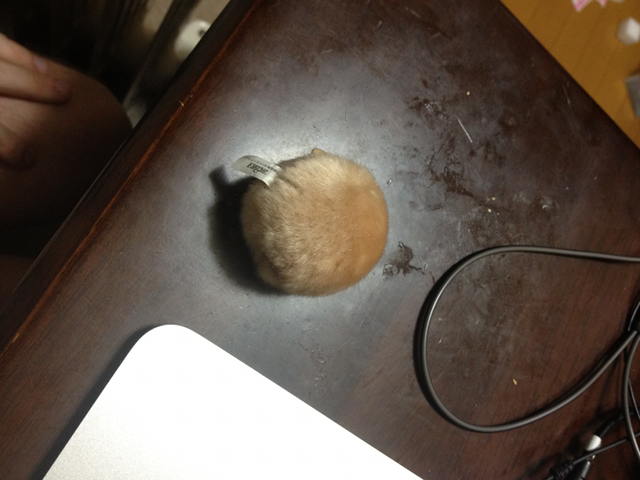
\includegraphics[height=1.5in]{images/tb2.png}
\label{s1}
	 } }
&
{
	 \subfloat[][]{
	   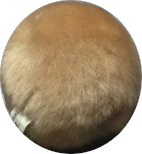
\includegraphics[height=1.5in]{images/t2.jpg}
\label{s2}
	 }}&
{
 \subfloat[][]{
	   
\includegraphics[height=1.5in]{images/test1.png}
\label{s3}
	 }}
\\[0.3in]

{\raisebox{0.75in}{Image set 2}}
&
{
 \subfloat[][]{
	   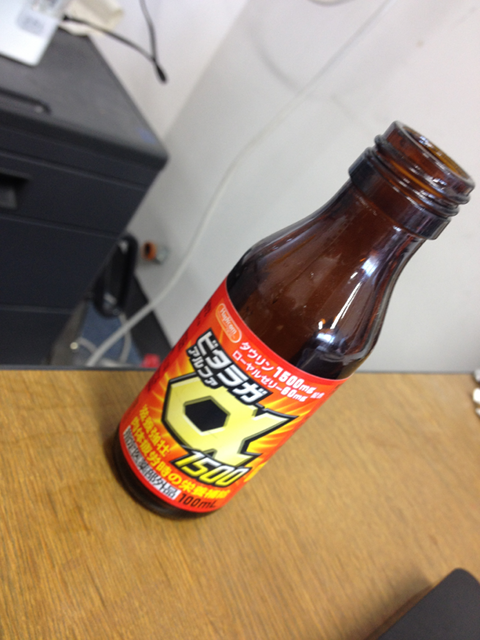
\includegraphics[height=1.5in]{images/train1.png}
\label{s4}
	 }}
&{
 \subfloat[][]{
	   
\includegraphics[height=1.5in]{images/ttext1.png}
\label{s5}
	 }}
&{
\subfloat[][]{
	   
\includegraphics[height=1.5in]{images/test2.png}
\label{s6}
	 }}

\end{tabular}
    \caption{Examples of training images and clipped textures. \protect \subref{s1} , \protect\subref{s4} Images used for training. \protect \subref{s2}, \protect \subref{s5}  Texture area extracted for training \protect \subref{s3}, \protect \subref{s6} Examples of the images used for evaluation.  
}
    \label{Samples1}
\end{figure*}
\begin{figure*}[t]

\begin{tabular}{|c||c|c|c||c|c|c|}

                                                                            \hline
   {}  &  \multicolumn{3}{|c||}{Image set 1}  &\multicolumn{3}{|c|}{Image set 2}    \\\hline
   {}  & {6 bits, 30 Ferns} & {8 bits, 30 Ferns}& {8 bits, 50 Ferns} &{6 bits, 30 Ferns}  &{8 bits, 30 Ferns}&{8 bits, 50 Ferns} \\\hline

 {log}  & {0.76} & {0.78}& {0.80} &{0.58}  &{0.57}&{0.58} \\\hline
 {prob}  & {0.51} & {0.52}& {0.61} &{0.5}  &{0.5}&{0.51} \\\hline
 {bin}  & {0.62} & {0.69}& {0.73} &{0.61}  &{0.61}&{0.63} \\\hline

 {wlog}  & {0.83} & {0.84}& {0.88} &{0.78}  &{0.81}&{0.90} \\\hline
 {wprob}  & {0.81} & {0.81}& {0.82} &{0.9}  &{0.9}&{0.92} \\\hline
 {wbin}  & {0.93} & {0.92}& {0.92} &{0.88}  &{0.89}&{0.92} \\\hline


{iwlog}  & {0.77} & {0.77}& {0.80} &{0.70}  &{0.75}&{0.80} \\\hline
 {iwprob}  & {0.60} & {0.63}& {0.75} &{0.81}  &{0.82}&{0.85} \\\hline
 {iwbin}  & {0.65} & {0.71}& {0.80} &{0.81}  &{0.83}&{0.85} \\\hline
\end{tabular}
\caption{Average ratio of successfully recognized pixels to the total number of pixels in the test image. Sample test images for the image sets 1 and 2 are presented on \ref{s3} and \ref{s6}, respectively.}
\label{tbl1}
\end{figure*}

We perform tests on the same set of images (examples given in Figure \ref{Samples1}), comparing accuracy of original Ferns and SVM-boosted ferns for 3 values of $l(F_k,c_i)$, for both interleaved and separate training phases. The averaged results of completed training are presented in table \ref{tbl1}.  It can be seen that all methods that use training provide increased accuracy over the original Ferns method, especially when the Ferns bit size and total amount of features are decreased. For particularly low values of fern size, the binary method starts to outperform other methods of likelihood estimation. This is useful for applications where the amount of storage is limited, since it allows storing each feature in single bits rather than floating point values. It should be noted that this increase of accuracy comes without any increase of computational cost during classification stage, since at most we only need to do additional $M$ multiplications per classification, while removing the need to calculate logarithms. 
To estimate the performance and accuracy of multiclass method, we perform the same tests as in the original Ferns article \cite{Ferns1}. The results are shown in Figure \ref{multires}. Our experiments have shown that while our algorithm outperforms the original on shorter Ferns and lower number of classes, benefits decrease as the amount of classes and available Ferns increases, indicating that for applications with larger available resources and stricter requirements to training times the original method could be preferable.

\begin{figure*}[t]
    \centering

	 \subfloat[][]{
	   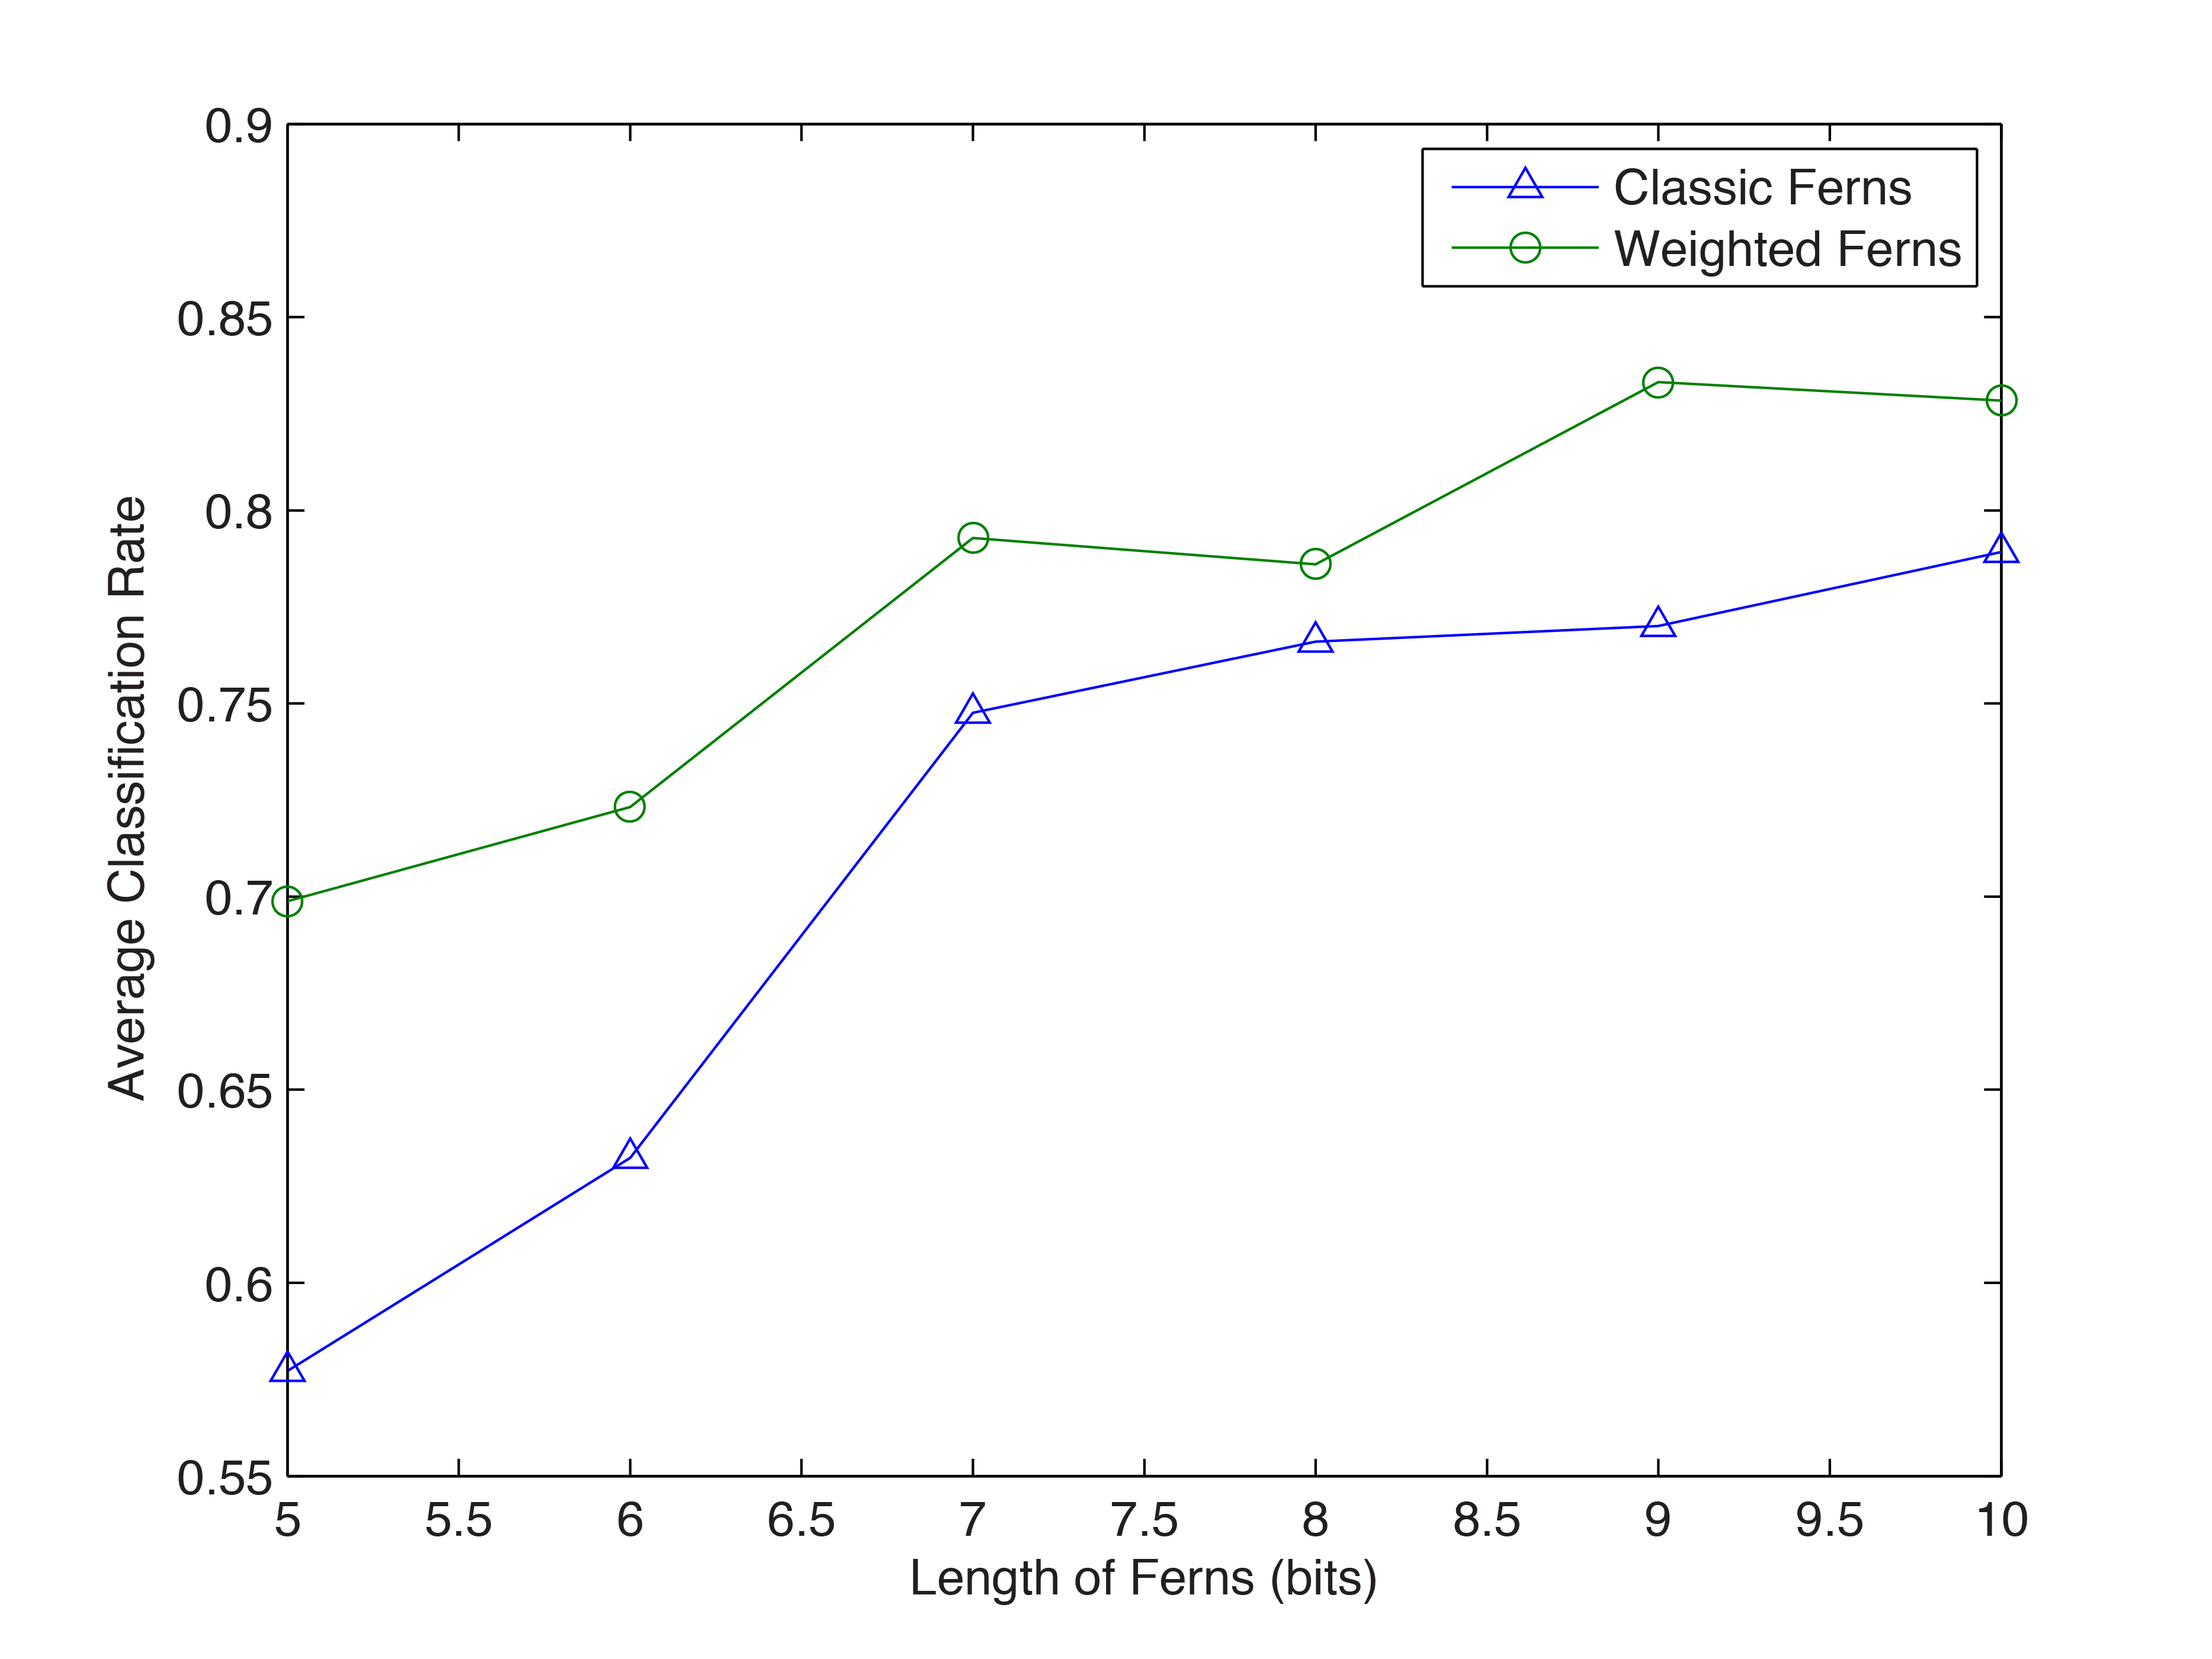
\includegraphics[height=2in]{images/fernlen.png}
\label{lenferns}
	 }
	 \subfloat[][]{
	   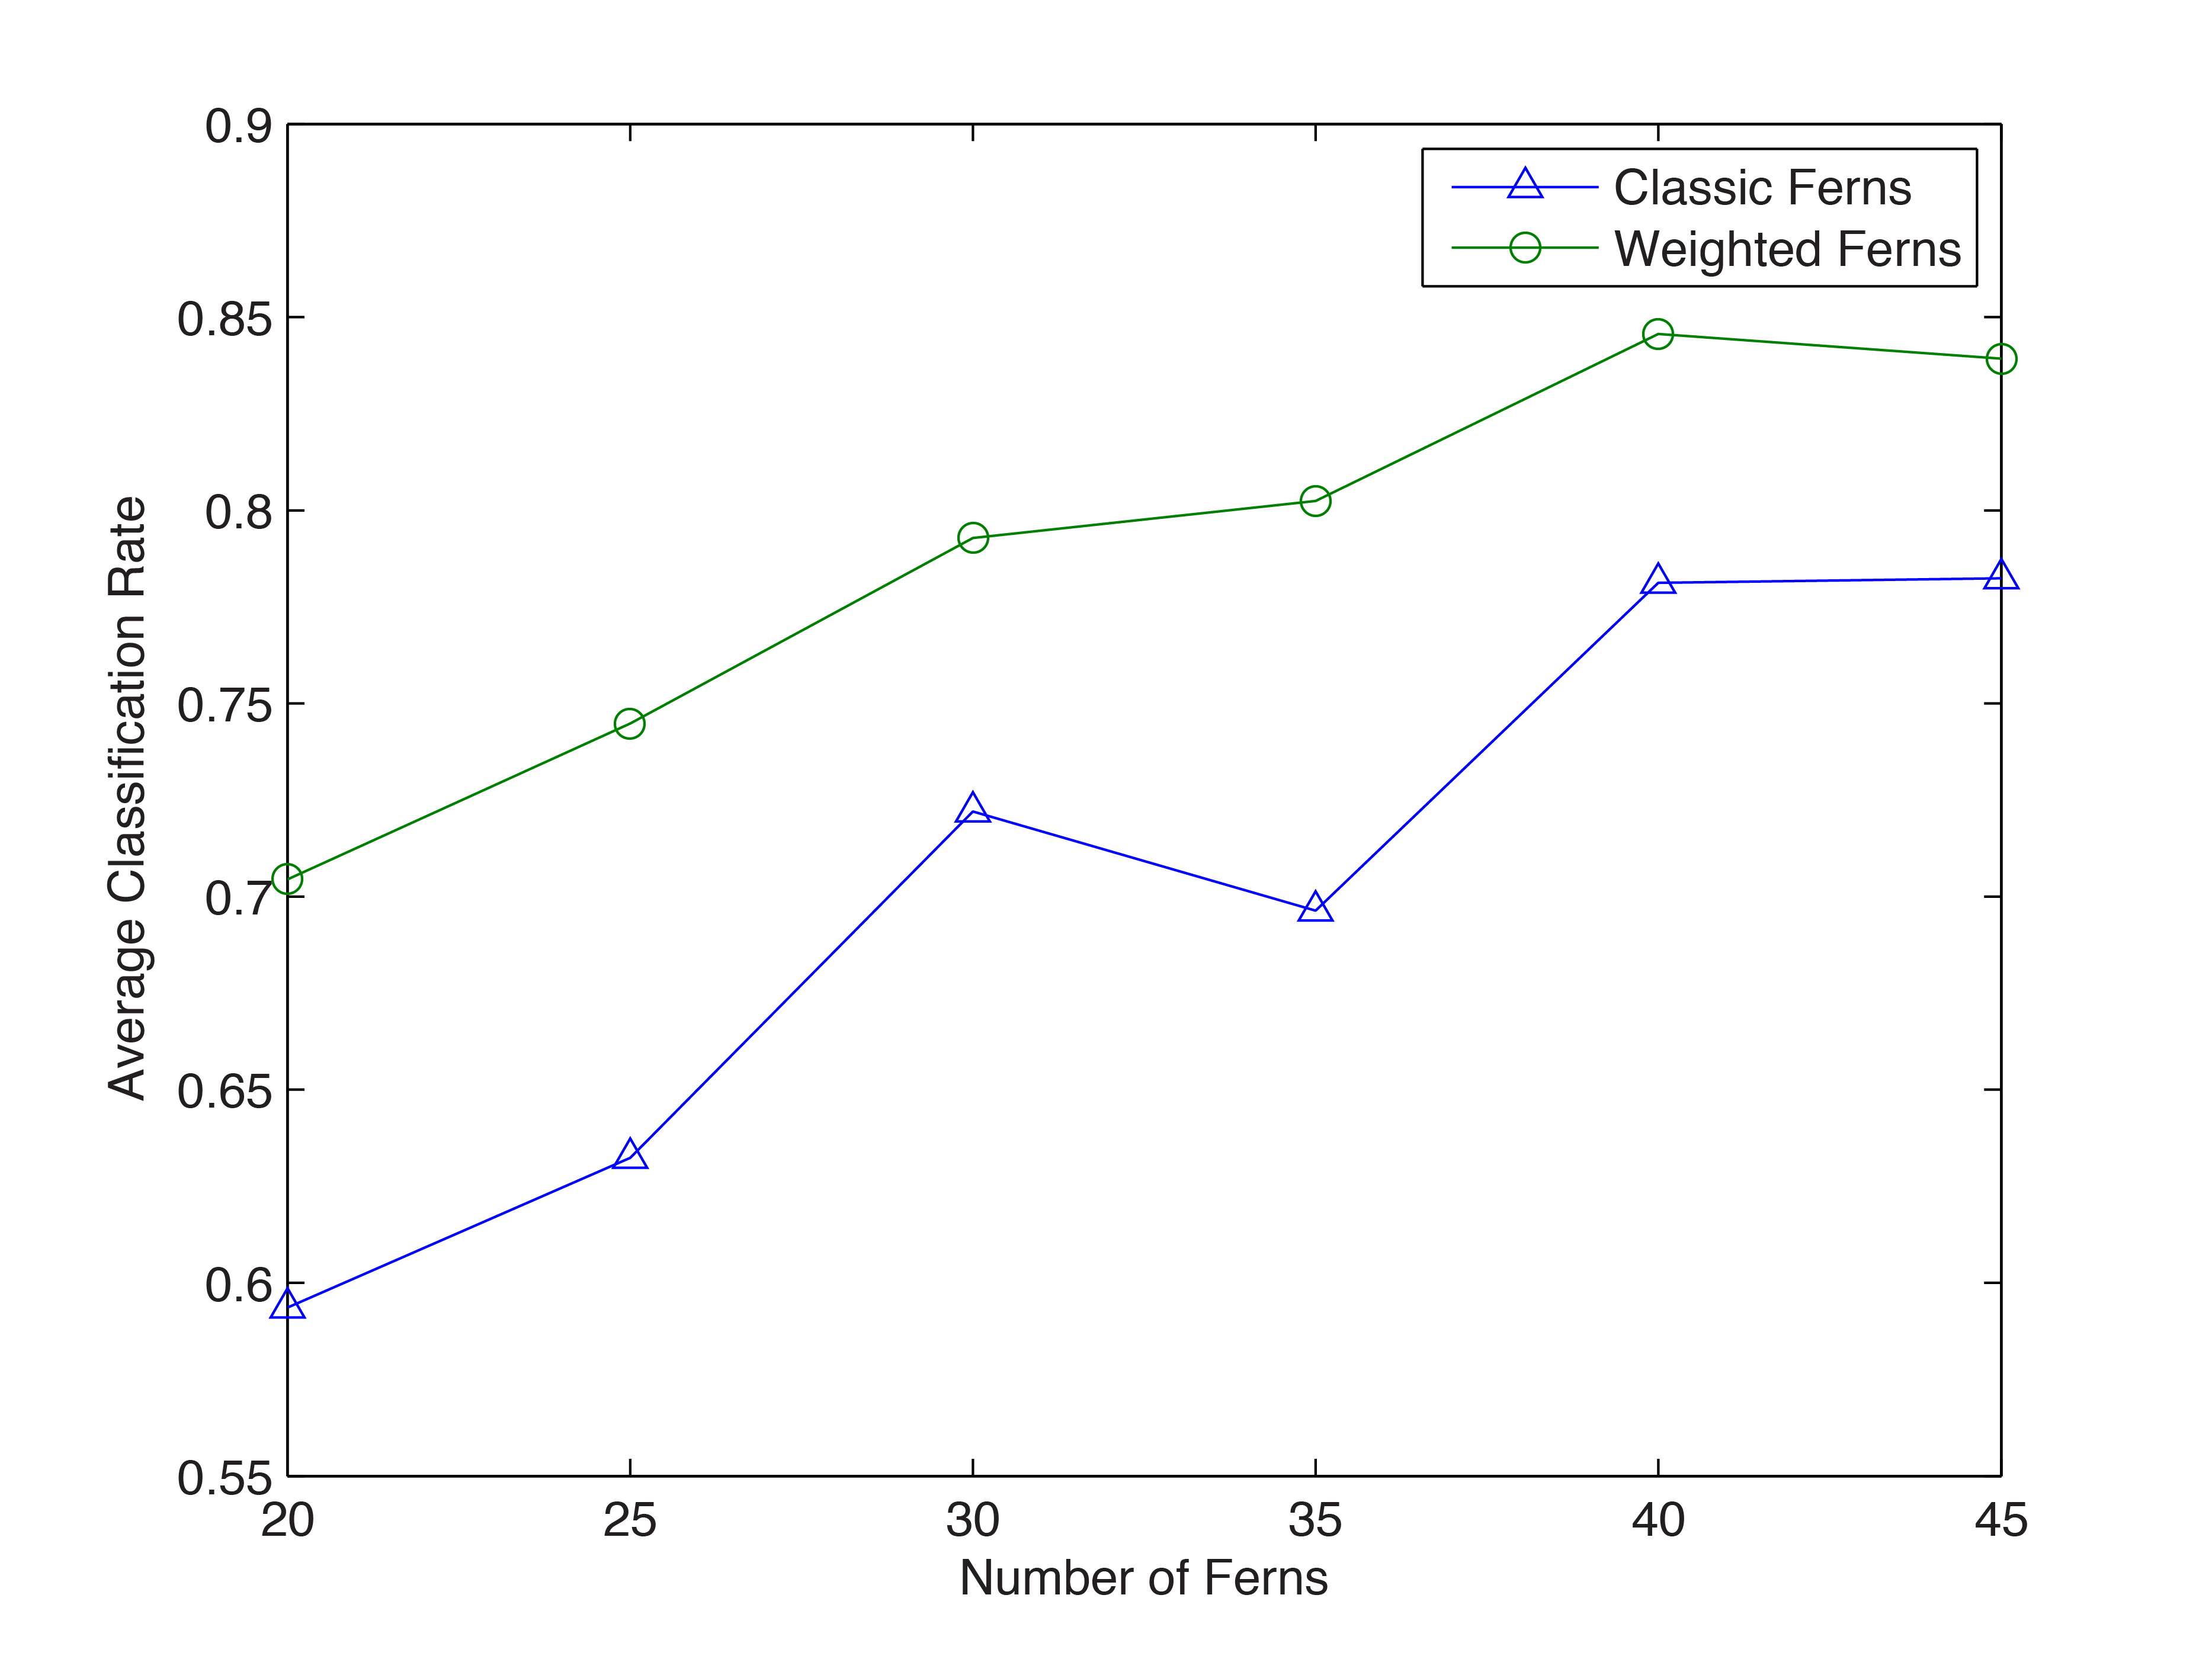
\includegraphics[height=2in]{images/fernnum.png}
\label{numferns}
}
  \caption{Results of testing multiclass approach described in section \ref{multiclass}.  Ratio of correctly classified image patches to a total number of patches (accuracy ratio). \protect \subref{lenferns}  Dependence of accuracy ratio on a bit length of each Fern (25 Ferns).  \protect\subref{numferns} Dependence of accuracy ratio on a total number of Ferns (8 bits per Fern).  }
\label{multires}
\end{figure*}

\section{Implementing GPU-accelerated version of the algorithm on a mobile device}
\label{implementation}
\begin{figure*}[t]

    \centering

	 \subfloat[][]{
	   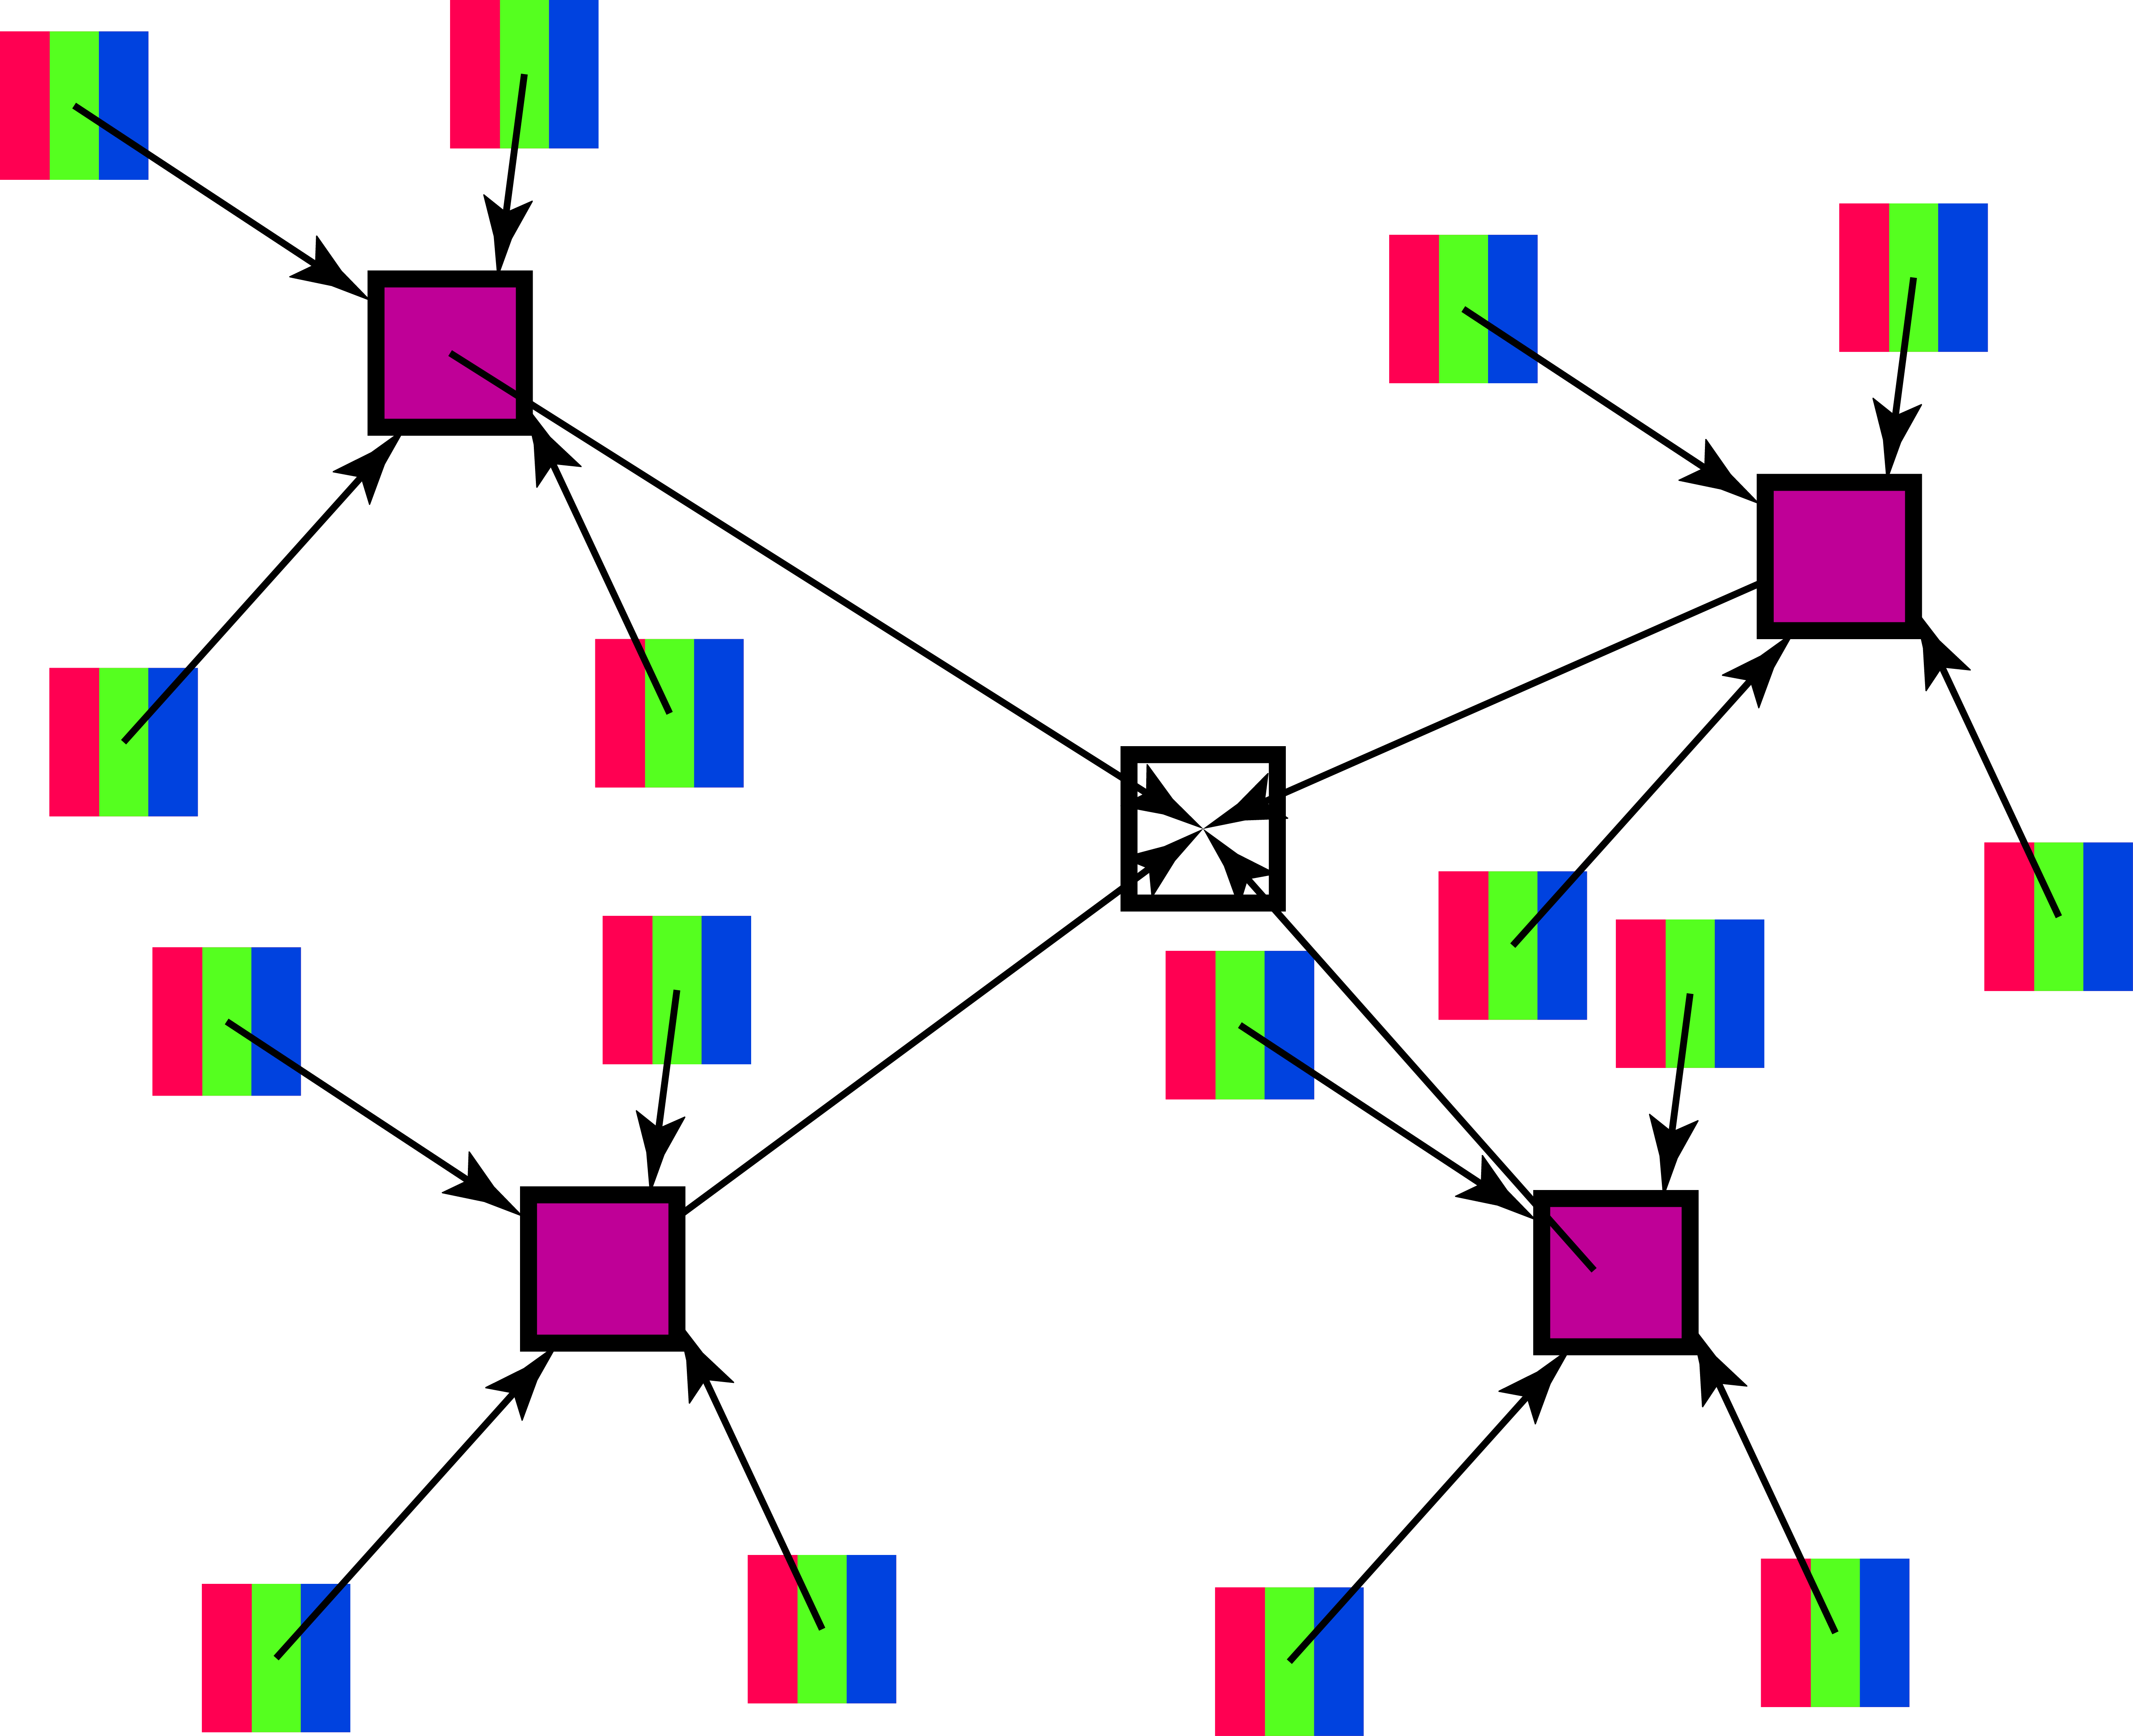
\includegraphics[height=2in]{images/Shader1c.png}
\label{eps1}
	 }
	 \subfloat[][]{
	   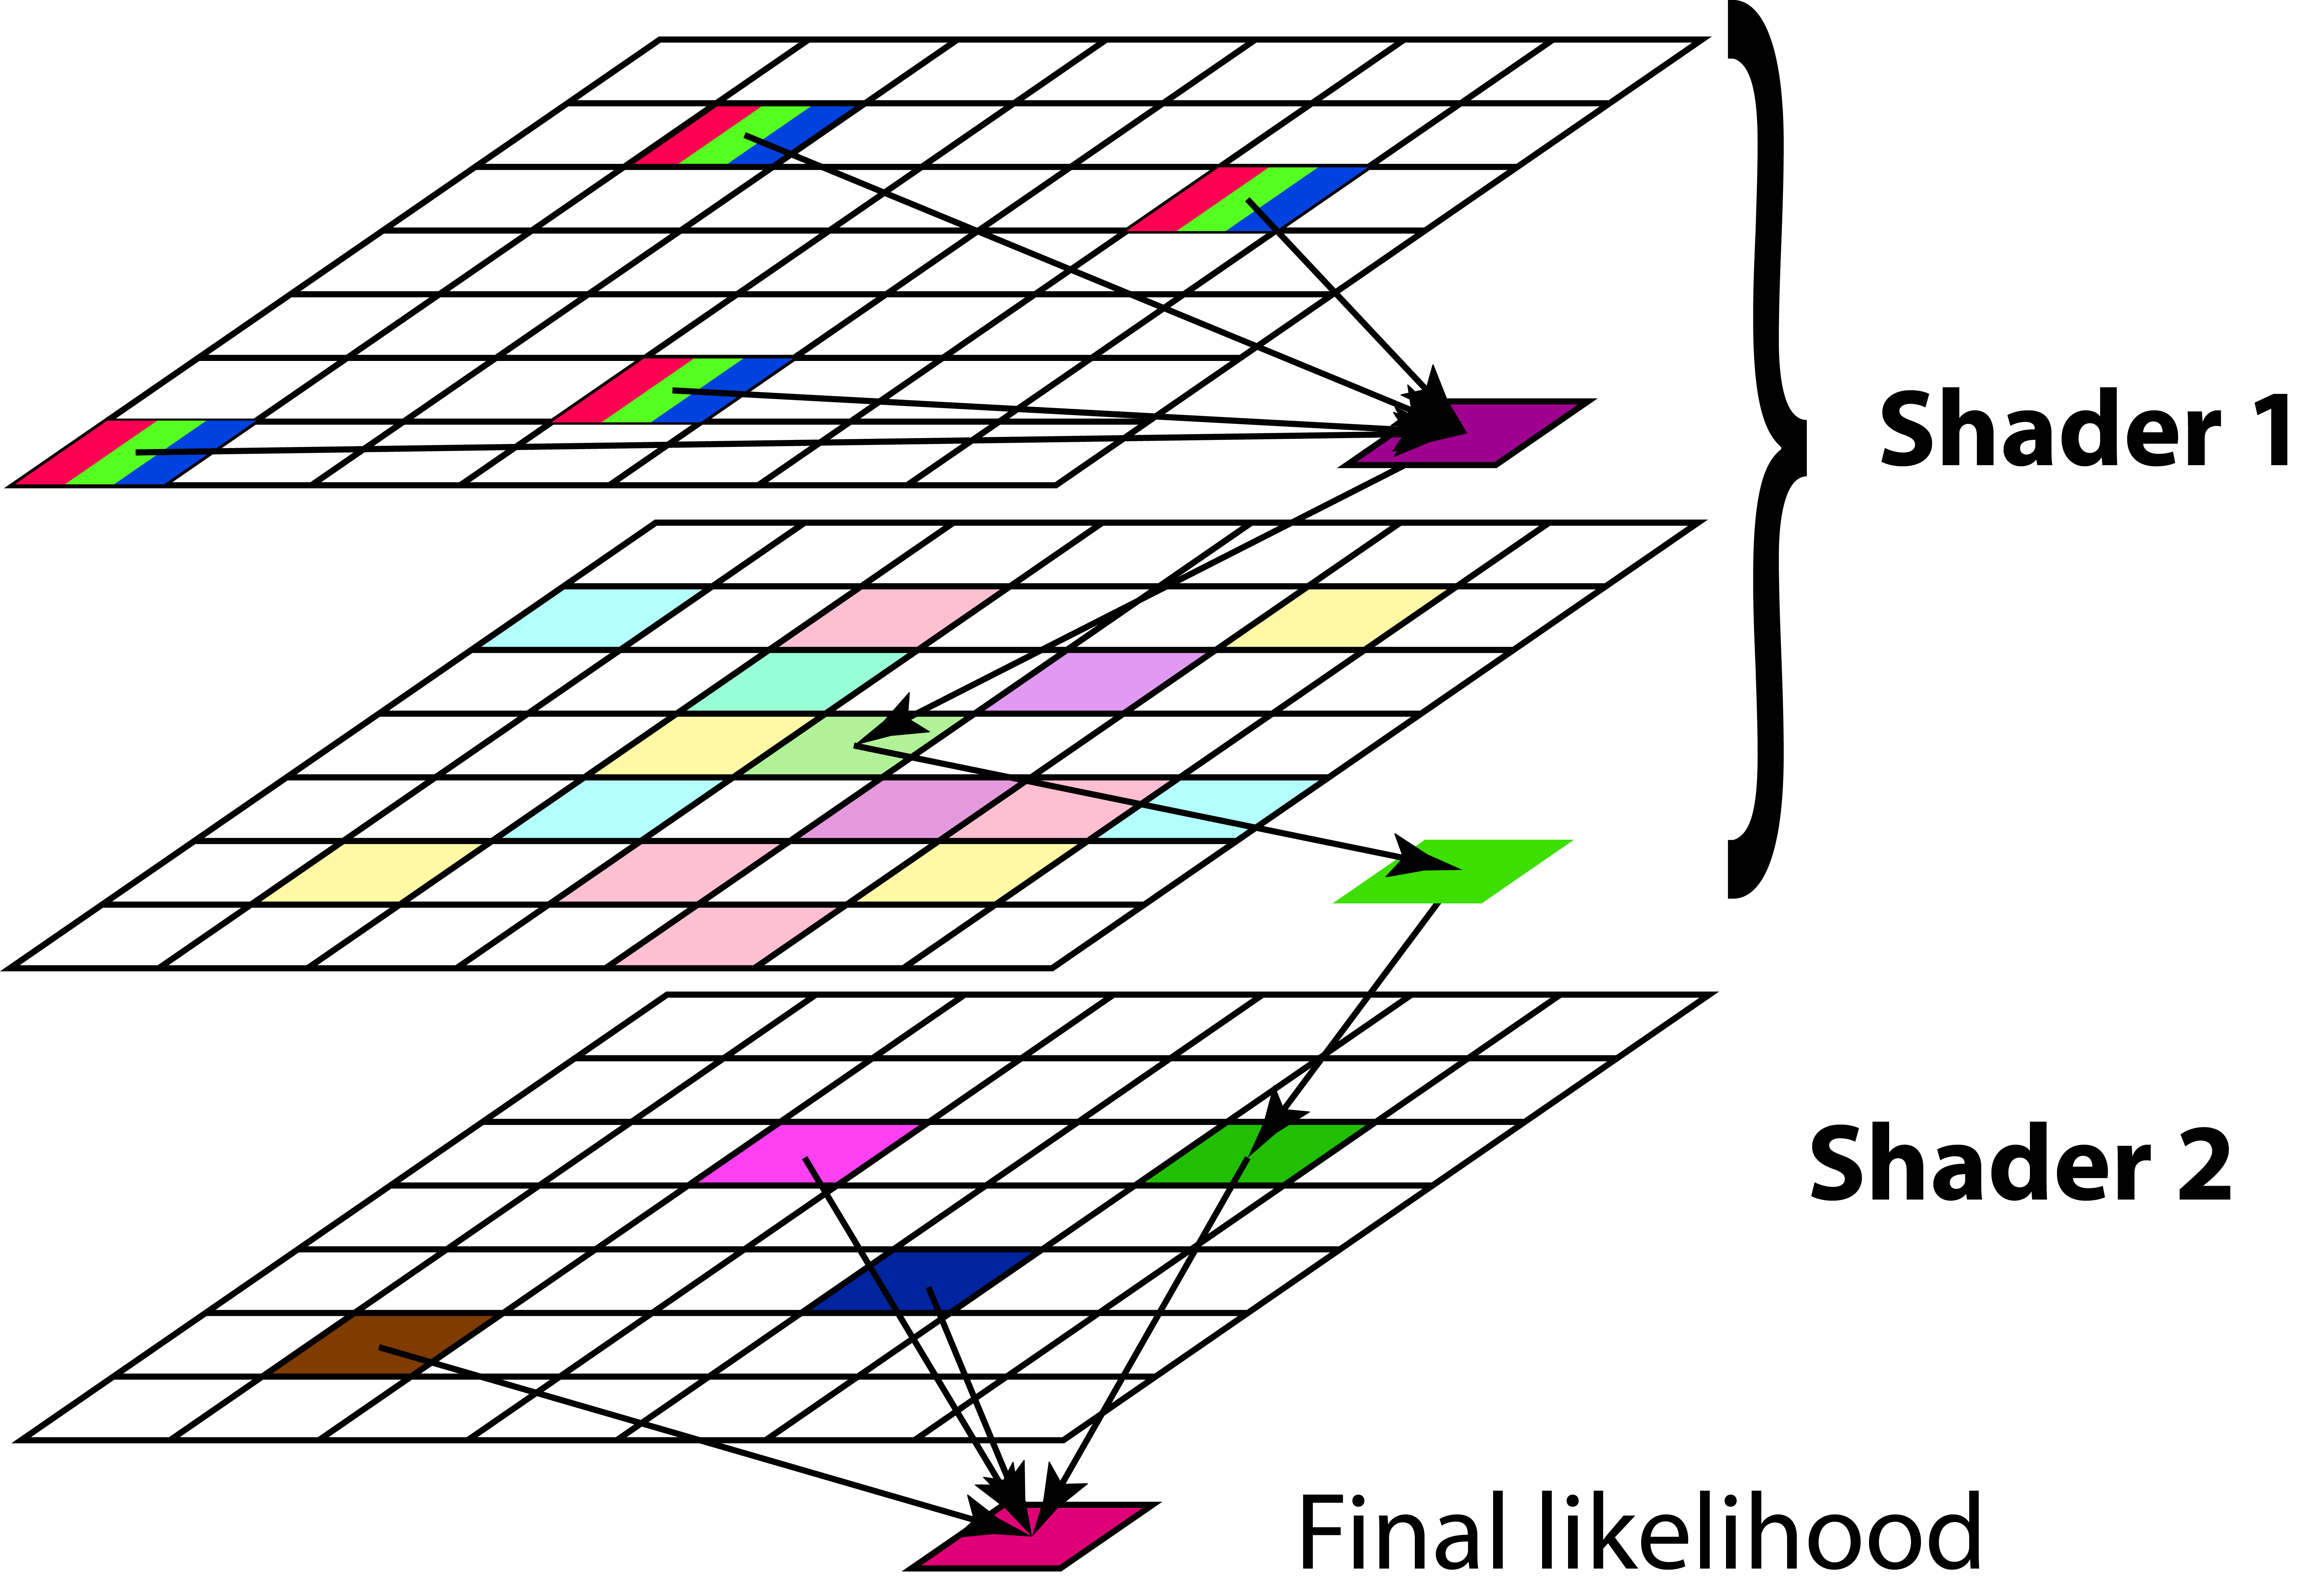
\includegraphics[height=2in]{images/Shader2c.png}
\label{eps2}
}

    \caption{ \protect \subref{eps1} Illustration of multilevel data aggregation. Four RGB pixels are processed by first layer, resulting in the intermediate value (purple). The next shader in chain then processes four intermediate values, aggregating data from a total of 16 pixels. \protect\subref{eps2} Illustration of complete shader chain for likelihood estimation. Shader 1 calculates Ferns and looks up premultiplied binary values in an auxiliary texture. Shader 2 aggregates outputs of Shader 1 into a single likelihood.}
\label{shaders}
\end{figure*}
Recently, GPGPU (general purpose GPU) programming is becoming popular, since it allows designing low-cost high-speed parallel computational solution. In the beginning, GPU computation has been confined to personal computers, since GPUs of mobile devices didn't allow custom programming. However, newer graphical libraries, such as now commonly used Open GL ES 2.0, allow the use of programmable shaders, small programs that run in parallel on GPU. In particular, fragment shaders, that run for each pixel of the output image, are well suited for image processing tasks. This has lead to an intensive research activity on using mobile GPU for high-speed image and video processing. For example \cite{gpusift1} considered implementing SIFT algorithm on the mobile phones with Android operating system. They conclude that while using both CPU and GPU increases the performance on mobile devices, mobile platform remains very restrictive and requires a lot of effort from the programmer but does not achieve the same performance gains as observed for the PC. These restrictions, unfortunately, remain for current generation of the mobile phones.
However, SIFT is not the best algorithm for parallel processing, though it certainly benefits from it. It requires repeated rescaling and convolving of the input image, and therefore uses a large amount of GPU iterations, increasing computational and memory costs. 
 In this section, we show ishow how to implement the texture recognition algorithm outlined in section \ref{malg}, based on two-class SVM-boosted Ferns. Its computation is performed mostly by GPU, with very little CPU participation. Since it allows estimating likelihood of a given pixel being part of texture are for every pixel of an image, the keypoint / ROI detection step can be avoided.
\subsection{Implementation details}
At its core, the implemented algorithm is simple. Once the offline training is done, we have a set of probability distributions and corresponding weights for all Ferns, which can then be arranged into lookup tables and saved as reference textures in the video memory. To simplify uploading process, tables are arranged and saved as PNG images beforehand (examples in Figure \ref{TSamples1}). Then, for classification, the fragment shader has to perform necessary binary tests to create Ferns for each pixel (using eq.  \ref{funct}), form lookup indices and calculate the resulting likelihoods by summing over values fetched from lookup texture. Here, however, we run into several limitations of the OpenGL ES shader programming.

1.	Relatively slow texture lookup. Looking up texel (texture element) values, especially when the coordinates are calculated in the fragment shader instead of being passed from vertex shader, is one of the most computationally expensive operations performed by GPU. Slow lookups limit the amount of binary tests that can be performed while maintaining real-time processing speed. It is therefore not possible to perform all binary feature evaluations and corresponding lookups necessary for Fern evaluation in the single shader.  The solution to this problem lies in separating evaluation into several stages, accumulating feature vectors and corresponding likelihood values over several iterations, as shown in Figure \ref{eps1}. The drawback to this technique lies in the fact that it introduces regularity in the feature offsets, limiting their randomness. This leads to additional dependence between separate Ferns, limiting contribution of each one in exchange for decreased computational costs. It also runs into a problem number of ouput constraints, outlined below. 

2.	 Memory constraints. The amount of available video memory on the mobile devices is extremely limited, especially considering large size of Fern lookup tables. Since they cannot be passed directly into the shader, in our implementation they are stored into an image and loaded into memory as a texture, introducing some ambiguity into the access routines, since transformation of the floating point coordinate values used in a shader to the integer texel coordinate is not exact. Still, as we show below, this does not affect the accuracy of the results. Also, to further reduce the amount of the memory necessary, we store binary values resulting from thresholding outlined in section \ref{malg} instead of actual probabilities, which allows us to reduce storage requirements up to 8 times. Unfortunately, several experiments have shown that the simplest way of data packing, i.e. storing data as individual bits in the 32-bit texels, is not feasible due to the lack of bitwise operation or integer texture support in OpenGL ES 2.0 specification. This forced us to use somewhat less efficient method of storing individual bits premultiplied by SVM coefficients in color channels. This allows us to store data about 4 Fern values and corresponding coefficients in a single texel, reducing the amount of texture fetches necessary and removing a multiplication operation from shader, reducing computaional load.

3.	Output constraints. The outputs of each fragment (pixel) shader in the OpenGL ES programming framework have to fit into a single pixel of the output texture, i.e. 4 bytes of data in floating point format, which is reduced to four 8-bit integers. Furthermore, the precision of floating point operations and variations in the driver implementation does not allow access to individual bits of the output. 


\subsection{Resulting algorithm}
\label{ra}
Our resulting algorithm uses chain of 2 shaders to transform original image into either likelihood estimation of each pixel belonging to an input texture or the thresholded value thereof.  The complete chain is illustrated in Figure \ref{eps2}. An additional shader is then used to blend the likelihoods with original image for visualization. As can be seen, all of the image processing is completely performed on the GPU, freeing up CPU for additional tasks, such as possible online model training.

\begin{figure}[t]
    \centering
\begin{minipage}{.25\textwidth}
	 \subfloat[][]{
	   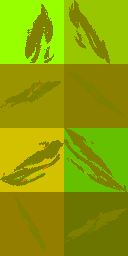
\includegraphics[height=1.5in]{images/bet4_1.png}
\label{ts:scr1}
	 }
	 \subfloat[][]{
	   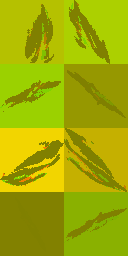
\includegraphics[height=1.5in]{images/bet4_2.png}
\label{ts:scr2}
	 }
	 \end{minipage}
	 \begin{minipage}{.2\textwidth}
 \subfloat[][]{
	   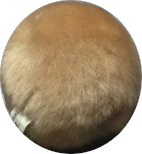
\includegraphics[height=0.7in]{images/t2.jpg}
\label{ts:scr3}
	 }\\
  \subfloat[][]{
	   
\includegraphics[height=0.7in]{images/backgrounds.png}
\label{ts:scr4}
	 }
	 \end{minipage}

    \caption{Weights and thresholded probabilitites encoded in two images (\protect \subref{ts:scr1} and \protect\subref{ts:scr2}) for loading in mobile device. Each square encodes two Ferns in red and green color channels. The length of each Fern is 10 bits, resulting in 32x32 square of two possible values, either 0 or the value of SVM coefficient corresponding to this Fern. \protect \subref{ts:scr3} Texture used for training \protect \subref{ts:scr1},\protect \subref{ts:scr2}. \protect \subref{ts:scr4} Sample of background used for training \protect \subref{ts:scr1}, \protect \subref{ts:scr2}.}
    \label{TSamples1}
\end{figure}

\subsection{Implementation results}
\label{iresults}

\begin{figure*}[t]
    \centering

	 \subfloat[][]{
	   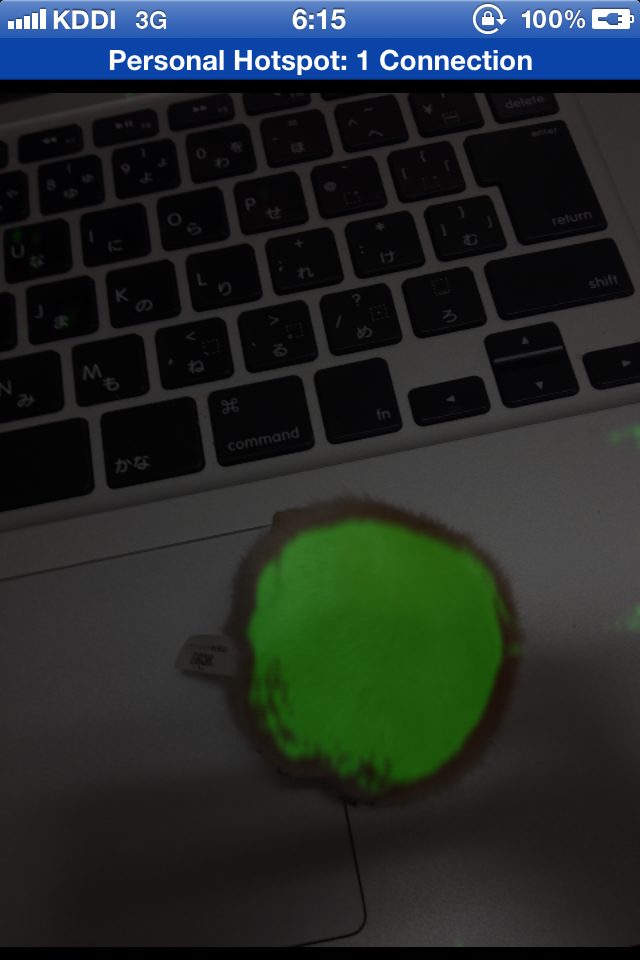
\includegraphics[width=0.25\textwidth]{images/IMG_1807.PNG}
\label{scre1}
	 }
	 \subfloat[][]{
	   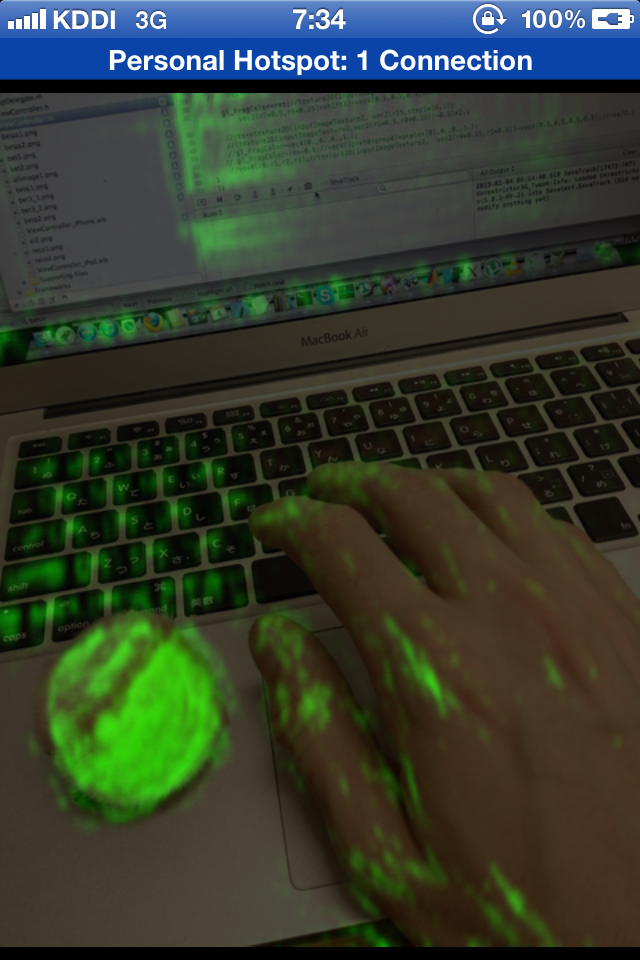
\includegraphics[width=0.25\textwidth]{images/IMG_1809.PNG}
\label{scre2}
	 }
 \subfloat[][]{
	   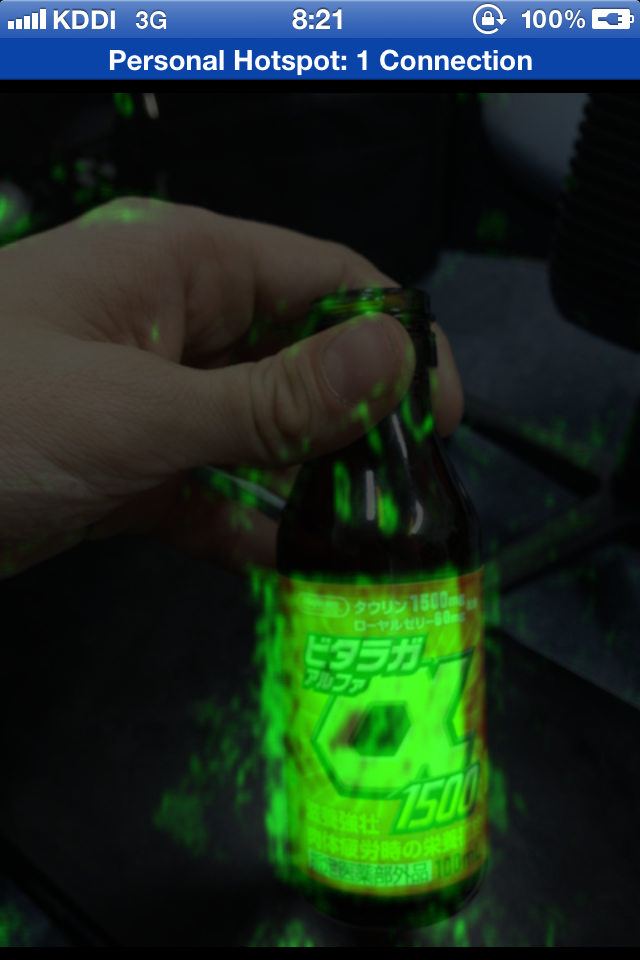
\includegraphics[width=0.25\textwidth]{images/IMG_1812.PNG}
\label{scre3}
	 }
 

    \caption{Screenshots of texture recognition algorithm in operation. \protect \subref{scre1} , \protect\subref{scre2} are results of using weighted Ferns trained on texture from Figure \protect \ref{s2}, \protect \subref{scre3} uses method trained on  Figure \protect \ref{s5}. }
    \label{screenshots}
\end{figure*}
Our algorithm with the above modifications was implemented on the iPhone4S. A built-in video camera, running at 30 fps with the resolution of 640x480, was used as source of input images. The two sets of images shown in Figure \ref{Samples1} were used separately  for training and recognition of the texture contained in each of them. The probability data from training was encoded in two png images each (example encoding images for 10-bit Ferns are presented in Figure \ref{TSamples1}, higher Fern length being used for improved clarity). For training, 64 6-bit ferns were used, and the joint distributions were then thresholded according to description in Section \ref{malg}. Since no ground truth values were available, the video was evaluated visually, and the speed of the algorithm was measured by averaging the time passing between frames. Several screenshots captured during the operation are displayed on Figure \ref {screenshots}. The average speed does not change with texture, remaining stable at about 0.04 seconds per frame, that is, algorithm allows us to achieve 25fps for a relatively high-resolution video.  As can be seen, our algorithm achieves high recognition accuracy for the trained texture despite change of pose, and achieves real-time speeds while processing all of the image pixels. 
\section{Conclusions and future work}
\label{conclusion}
We introduce an algorithm to increase accuracy of methods based on semi-naive Bayesian approach, with the goal of using such methods for real-time image processing under computational limitation of CPU, Memory and GPU of a mobile device. Specifically, we modified Ferns algorithm to work with the support vector machine framework to combine estimated joint probabilities into class likelihood. The resulting algorithm keeps the simplicity and scalability of the Ferns algorithm and further achieves an increase in accuracy for applications with a lower number of features. The algorithm was also modified to allow texture recognition. This in turn allows us to implement proposed algorithm completely on a mobile device GPU, achieving high speed processing of 640x480 video feed, while maintaining an acceptable degree of accuracy.


\bibliographystyle{plain}
\bibliography{SVANew}
\end{document} 